% EDCCS 2026 — Presentation Slides
% Active Inference for Multi-Stream Edge Video Orchestration under Partial Observability
\documentclass[aspectratio=169,10pt]{beamer}

% ---------- Theme / Colors -----------------------------------------------
\usetheme{default}
\setbeamertemplate{navigation symbols}{}
\setbeamertemplate{footline}{%
  \hfill\insertframenumber\,/\,\inserttotalframenumber\hspace{8pt}\vspace{4pt}
}
\setbeamertemplate{itemize item}{\textbullet}
\setbeamertemplate{itemize subitem}{--}

\definecolor{myblue}{RGB}{26,55,115}
\definecolor{myaccent}{RGB}{0,130,140}
\definecolor{mywarn}{RGB}{192,57,43}
\definecolor{mygreen}{RGB}{26,120,58}
\definecolor{mygray}{RGB}{90,90,90}

\setbeamercolor{structure}{fg=myblue}
\setbeamercolor{frametitle}{bg=myblue,fg=white}
\setbeamercolor{title}{bg=myblue,fg=white}
\setbeamercolor{subtitle}{fg=white}
\setbeamercolor{author}{fg=white}
\setbeamercolor{institute}{fg=white!85}
\setbeamercolor{date}{fg=white!75}
\setbeamercolor{block title}{bg=myblue!90,fg=white}
\setbeamercolor{block body}{bg=myblue!6}
\setbeamercolor{alerted text}{fg=mywarn}
\setbeamercolor{alerted block title}{bg=mywarn,fg=white}
\setbeamercolor{alerted block body}{bg=mywarn!8}
\setbeamercolor{example text}{fg=mygreen}

% ---------- Packages -----------------------------------------------------
\usepackage[T1]{fontenc}
\usepackage[utf8]{inputenc}
\usepackage{graphicx}
\usepackage{amsmath,amssymb}
\usepackage{booktabs}
\usepackage{xcolor}
\usepackage{tikz}
\usetikzlibrary{arrows.meta,positioning,fit,backgrounds}

% ---------- Title info ---------------------------------------------------
\title{Active Inference for Multi-Stream\\
       Edge Video Orchestration\\
       under Partial Observability}
\author{[Author Name] \and Schahram Dustdar}
\institute{TU Wien, Vienna, Austria}
\date{EDCCS 2026 @ ICDCS \\ Seoul, June 2026}

% =========================================================================
\begin{document}

% ---- Title slide --------------------------------------------------------
\begin{frame}[plain]
\titlepage
\end{frame}

% ---- 1. The Question ----------------------------------------------------
\begin{frame}{The Question}
\vspace{0.6cm}
\begin{center}
  {\LARGE
  ``When the true GPU load state is hidden from the scheduler,\\[0.45em]
  should it \emph{react} to noisy FPS and latency signals directly —\\[0.45em]
  or first \textbf{infer the hidden state}, then act?''
  }
\end{center}
\vfill
\begin{center}
  \textcolor{myblue!50}{\rule{11cm}{0.5pt}}\\[0.4em]
  \textcolor{mygray}{
    This paper: formulate as POMDP $\;\cdot\;$ deploy Active Inference on real hardware $\;\cdot\;$\\
    empirically isolate \emph{what actually drives performance}
  }
\end{center}
\end{frame}

% ---- 2. Setup -----------------------------------------------------------
\begin{frame}{The Setup — Three-Node Edge Cluster}
\begin{columns}[T]
  \begin{column}{0.56\textwidth}
    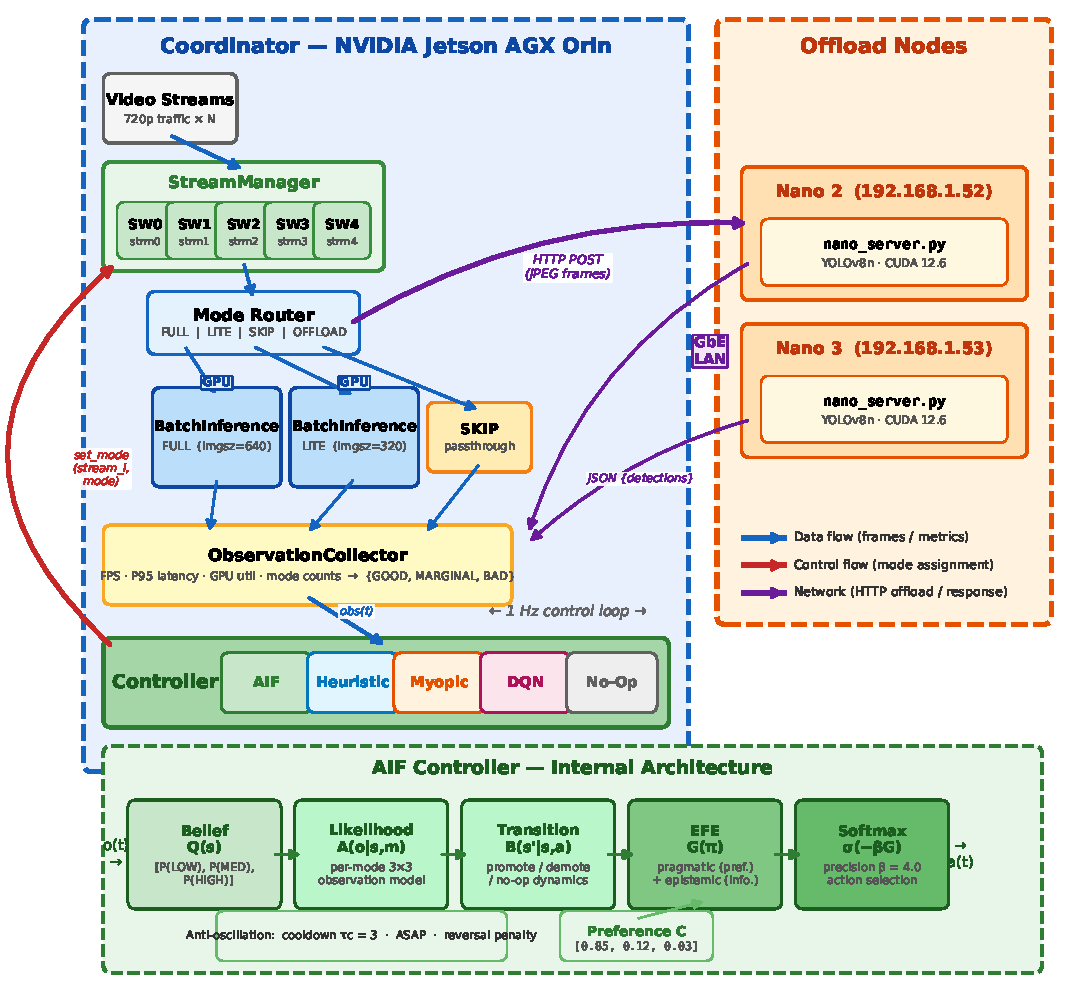
\includegraphics[width=\textwidth]{figures/architecture.pdf}
  \end{column}
  \begin{column}{0.41\textwidth}
    \vspace{0.3cm}
    \textbf{Hardware:}\\
    3$\times$ Jetson Orin Nano 8\,GB (1024 CUDA cores)\\
    1 coordinator + 2 stateless offload workers\\[0.55em]
    \textbf{Workload:}\\
    YOLOv8n on 720p video, up to 7 concurrent streams\\[0.55em]
    \textbf{Four execution modes per stream:}
    \begin{itemize}\setlength\itemsep{2pt}
      \item \textbf{FULL} — 640px, highest quality, highest GPU cost
      \item \textbf{LITE} — 320px, lower GPU cost
      \item \textbf{SKIP} — no inference, zero GPU, zero detections
      \item \textbf{OFFLOAD} — HTTP POST to worker ($\leq$2 concurrent)
    \end{itemize}
    \vspace{0.5em}
    \textbf{SLO target:} FPS\,$\geq$\,10, P95\,$\leq$\,150\,ms\\
    \textbf{Control loop:} 1-second steps
  \end{column}
\end{columns}
\end{frame}

% ---- 3. The Problem -----------------------------------------------------
\begin{frame}{GPU Contention Is Real}
\begin{columns}[T]
  \begin{column}{0.65\textwidth}
    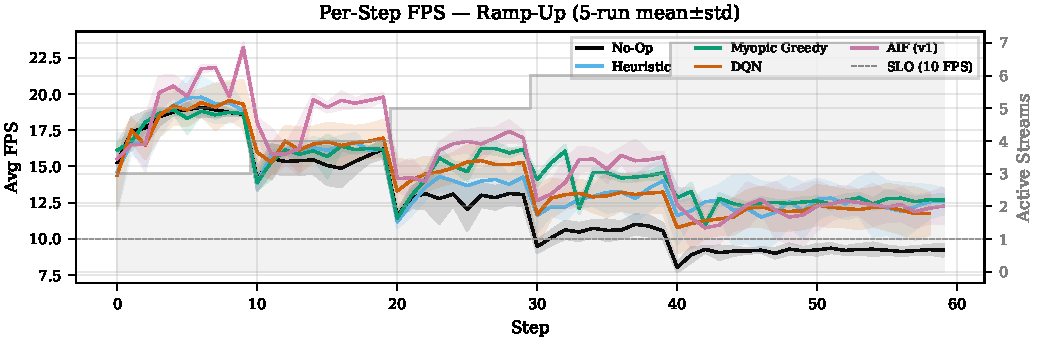
\includegraphics[width=\textwidth]{figures/fig_ts_fps_scenario_ramp_up.pdf}
  \end{column}
  \begin{column}{0.32\textwidth}
    \vspace{0.4cm}
    \small\textit{Ramp-up: streams added one-by-one, 3\,$\to$\,7 over 60\,s}\\[0.8em]
    \textbf{The inflection point:}\\[0.2em]
    5 streams\,$\to$\,\textcolor{mygreen}{\textbf{10.6 FPS ✓}}\\[0.15em]
    6 streams\,$\to$\,\textcolor{mywarn}{\textbf{8.7 FPS ✗}}\\[0.8em]
    \textbf{No-Op} (black) drops below the 10\,FPS SLO line at step\,$\approx$\,20 and never recovers.\\[0.7em]
    A scheduler must act.\\[0.3em]
    \textit{But reacting to what?}
  \end{column}
\end{columns}
\end{frame}

% ---- 4. Why Hard — POMDP ------------------------------------------------
\begin{frame}{Why Is This Hard? — It's a POMDP}
\begin{center}
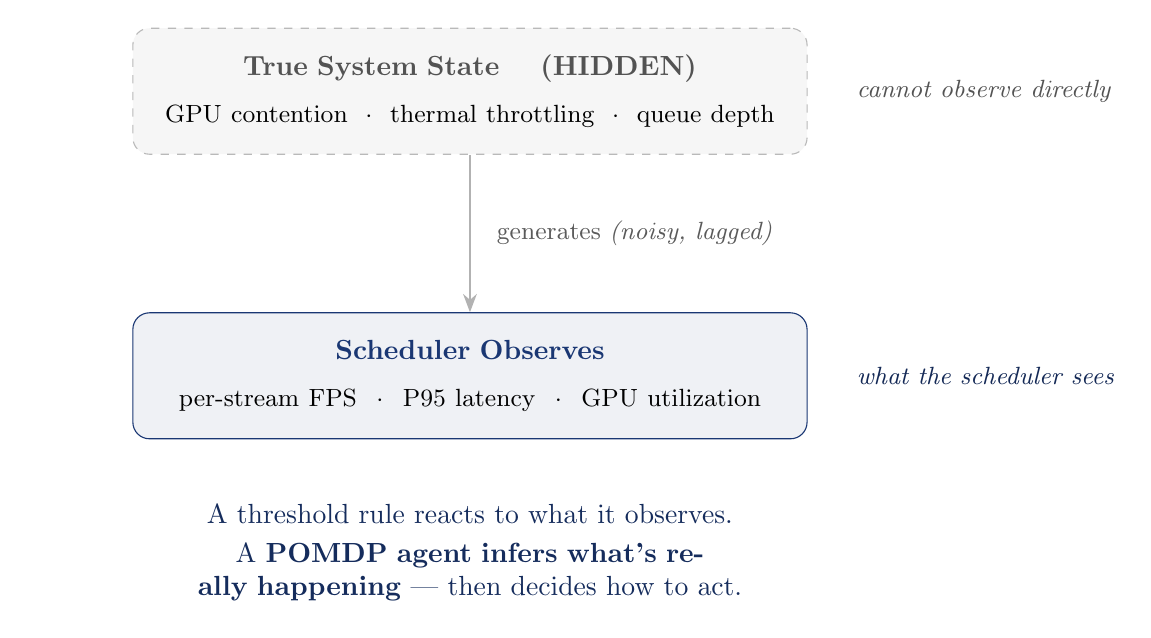
\begin{tikzpicture}[>=Stealth, font=\normalsize, node distance=1.8cm]

  \node[draw=gray!55, dashed, fill=gray!7, rounded corners=6pt,
        text width=8cm, minimum height=1.6cm, align=center, inner sep=8pt]
        (hidden) at (0, 0) {
    {\bfseries\color{gray!65!black} True System State \quad (HIDDEN)}\\[5pt]
    \small GPU contention $\;\cdot\;$ thermal throttling $\;\cdot\;$ queue depth
  };

  \node[draw=myblue, fill=myblue!7, rounded corners=6pt,
        text width=8cm, minimum height=1.6cm, align=center, inner sep=8pt,
        below=2cm of hidden] (obs) {
    {\bfseries\color{myblue} Scheduler Observes}\\[5pt]
    \small per-stream FPS $\;\cdot\;$ P95 latency $\;\cdot\;$ GPU utilization
  };

  \draw[-{Stealth}, thick, gray!60]
        (hidden) -- node[right=6pt, font=\small, text=mygray]
        {generates \textit{(noisy, lagged)}} (obs);

  \node[right=0.5cm of hidden, font=\small\itshape, text=gray!65!black]
        {cannot observe directly};
  \node[right=0.5cm of obs,    font=\small\itshape, text=myblue!75!black]
        {what the scheduler sees};

  \node[below=0.7cm of obs, text width=11cm, align=center,
        font=\normalsize, text=myblue!80!black] {
    A threshold rule reacts to what it observes.\\[2pt]
    A \textbf{POMDP agent infers what's really happening} — then decides how to act.
  };

\end{tikzpicture}
\end{center}
\end{frame}

% ---- 5. Generative Model Construction -----------------------------------
\begin{frame}{Building the Generative Model}
\begin{columns}[T]

  %% Left — component table
  \begin{column}{0.36\textwidth}
    \vspace{0.2cm}
    \small
    \begin{tabular}{@{}p{0.9cm}p{3.8cm}@{}}
      \toprule
      \textbf{Comp.} & \textbf{What it encodes} \\
      \midrule
      $A(o|s,m)$   & Obs.\ likelihood per mode\\
                   & $3{\times}3$ per action \\\addlinespace
      $B(s'|s,a)$  & State transition dynamics\\
                   & demote / promote / no-op \\\addlinespace
      $C(o)$       & Preferred observations\\
                   & $[0.85,\;0.12,\;0.03]$ \\\addlinespace
      $D(s)$       & Prior belief\\
                   & uniform $[1/3,\;1/3,\;1/3]$ \\
      \bottomrule
    \end{tabular}
    \vspace{0.5em}

    \footnotesize\textcolor{mygray}{
      $B$, $C$, $D$: hand-specified from\\
      domain knowledge and SLO spec.\\[0.3em]
      All design complexity is in $A$.
    }
  \end{column}

  %% Right — how A is constructed
  \begin{column}{0.61\textwidth}
    \vspace{0.1cm}
    \small\textbf{\textcolor{myblue}{How are the $A$ matrices constructed?}}
    \vspace{0.35cm}

    \begin{columns}[T]
      \begin{column}{0.48\textwidth}
        \setbeamercolor{block title}{bg=myaccent!80,fg=white}
        \setbeamercolor{block body}{bg=myaccent!8}
        \begin{block}{Hardware profiling}
          \footnotesize
          Run YOLOv8n at 1–7 concurrent streams.\\
          Measure FPS and P95 latency.\\
          Bin into GOOD / MARG / BAD.\\[5pt]
          $\Rightarrow$ $A^{\textsc{Full}}$, $A^{\textsc{Lite}}$
        \end{block}
      \end{column}
      \begin{column}{0.48\textwidth}
        \setbeamercolor{block title}{bg=mygreen!80,fg=white}
        \setbeamercolor{block body}{bg=mygreen!8}
        \begin{block}{Causal reasoning}
          \footnotesize
          OFFLOAD benefits \emph{other} streams\\
          — cannot be directly profiled.\\[2pt]
          SKIP = degraded service,\\
          coverage cost regardless of state.\\[5pt]
          $\Rightarrow$ $A^{\textsc{Offload}}$\,v1, $A^{\textsc{Skip}}$\,mod.
        \end{block}
      \end{column}
    \end{columns}

    \vspace{0.45cm}
    \setbeamercolor{block title}{bg=mywarn!80,fg=white}
    \setbeamercolor{block body}{bg=mywarn!7}
    \begin{block}{}
      \footnotesize\centering
      Profiling gives \textbf{local} observations.\quad
      Causal reasoning gives \textbf{system-level} consequences.\\[3pt]
      The causal matrices drive \textbf{+14.4 pp} —
      the profiling matrices are necessary but not sufficient.
    \end{block}
  \end{column}

\end{columns}
\end{frame}

% ---- 6. Core Idea -------------------------------------------------------
\begin{frame}{The Core Idea — Encode What Actions Actually Do}
\begin{columns}[T]
  \begin{column}{0.55\textwidth}
    \vspace{0.1cm}
    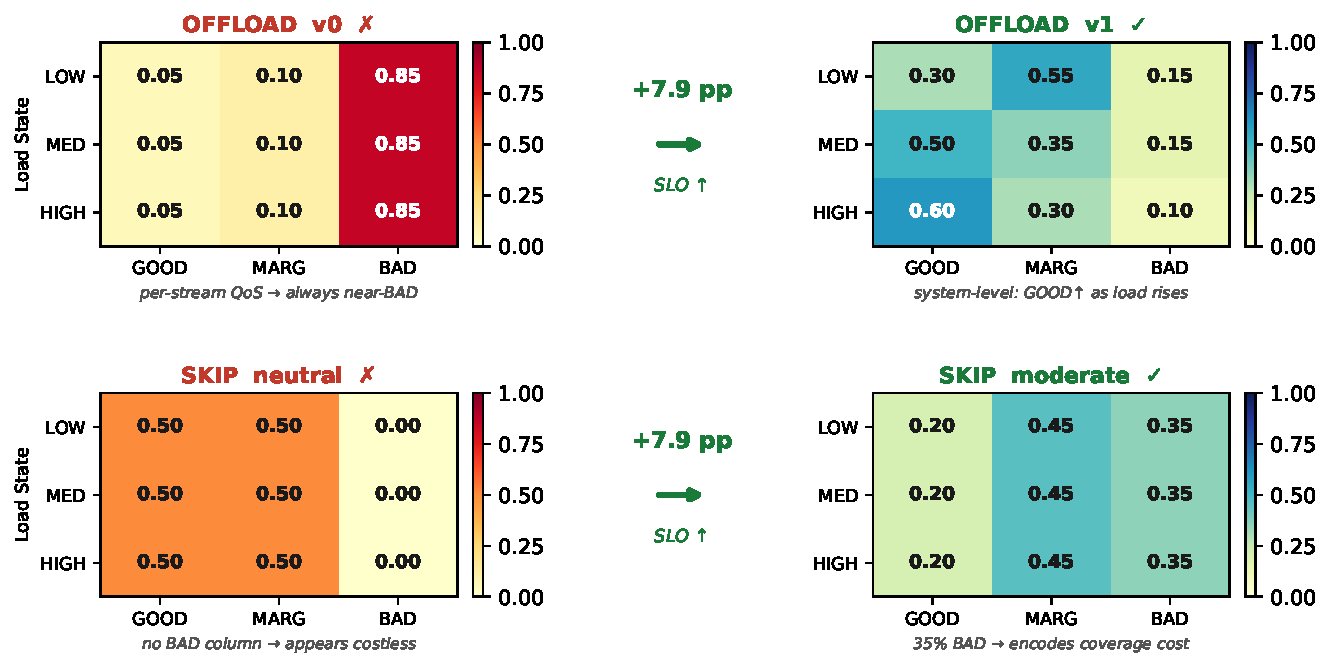
\includegraphics[width=\textwidth]{figures/fig_encoding_comparison.pdf}
  \end{column}
  \begin{column}{0.42\textwidth}
    \vspace{0.25cm}
    \small
    \textbf{\textcolor{mywarn}{OFFLOAD v0 (wrong):}}\\
    Model uses the offloaded stream's own FPS ($\sim$7, near-BAD).\\
    Controller thinks OFFLOAD is always a bad action\\
    $\to$ never uses it. \quad 0\% offload ratio.\\[0.6em]

    \textbf{\textcolor{mygreen}{OFFLOAD v1 (right):}}\\
    Offloading frees local GPU capacity.\\
    Remaining streams improve — \emph{that} effect goes in the model.\\
    \hspace{1em}\textbf{\textcolor{mygreen}{+7.9 pp SLO}}\\[0.6em]

    \textbf{\textcolor{mywarn}{SKIP neutral (wrong):}}\\
    SKIP has no BAD in the likelihood.\\
    Appears costless $\to$ overused (13\% skip ratio).\\[0.6em]

    \textbf{\textcolor{mygreen}{SKIP moderate (right):}}\\
    SKIP = degraded service. 35\% BAD encodes coverage cost.\\
    \hspace{1em}\textbf{\textcolor{mygreen}{+7.9 pp SLO}}\\[0.5em]

    \begin{block}{}
    \footnotesize\centering
    Model construction, not algorithm choice,\\
    is the primary challenge.
    \end{block}
  \end{column}
\end{columns}
\end{frame}

% ---- 6. AIF in one picture ----------------------------------------------
\begin{frame}{AIF in One Picture — How It Works}
\begin{columns}[T]
  \begin{column}{0.56\textwidth}
    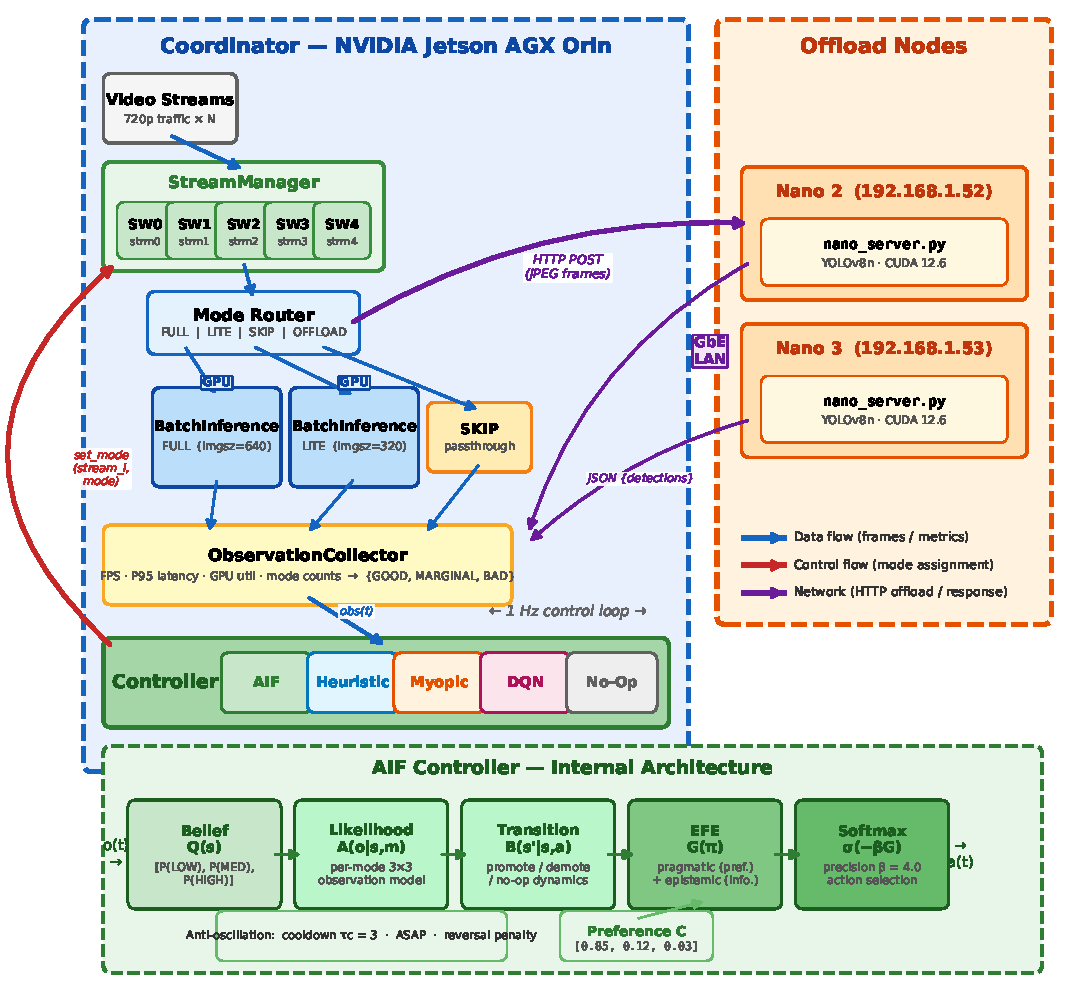
\includegraphics[width=\textwidth]{figures/architecture.pdf}
  \end{column}
  \begin{column}{0.41\textwidth}
    \vspace{0.3cm}
    \small
    \textbf{At each 1-second step:}
    \begin{enumerate}\setlength\itemsep{4pt}
      \item \textbf{Belief update} $Q(s)_t$\\
            Bayesian update from noisy observation:\\
            $Q(s)_t \propto A^{m}_{s,\,o_t}\cdot Q(s)_{t-1}$
      \item \textbf{EFE per action:}\\
            $G(a) = \underbrace{-\mathbb{E}[\ln C(o)]}_{\text{pragmatic}}
                   \;-\;\underbrace{w_e\cdot\mathrm{KL}[\cdot]}_{\text{epistemic}}$
      \item \textbf{Action selection}\\
            Precision-weighted softmax ($\beta = 4.0$)
    \end{enumerate}
    \vspace{0.6em}
    \textbf{Engineering approximation:}\\
    T\,=\,1 (single-step EFE). $<$1\,ms/step on Jetson.\\
    Belief $Q(s)$ carries forward history.\\[0.5em]
    \textbf{No training data. Works from step one.}
  \end{column}
\end{columns}
\end{frame}

% ---- 7. Four scenarios --------------------------------------------------
\begin{frame}{Four Workload Scenarios}
\begin{center}
  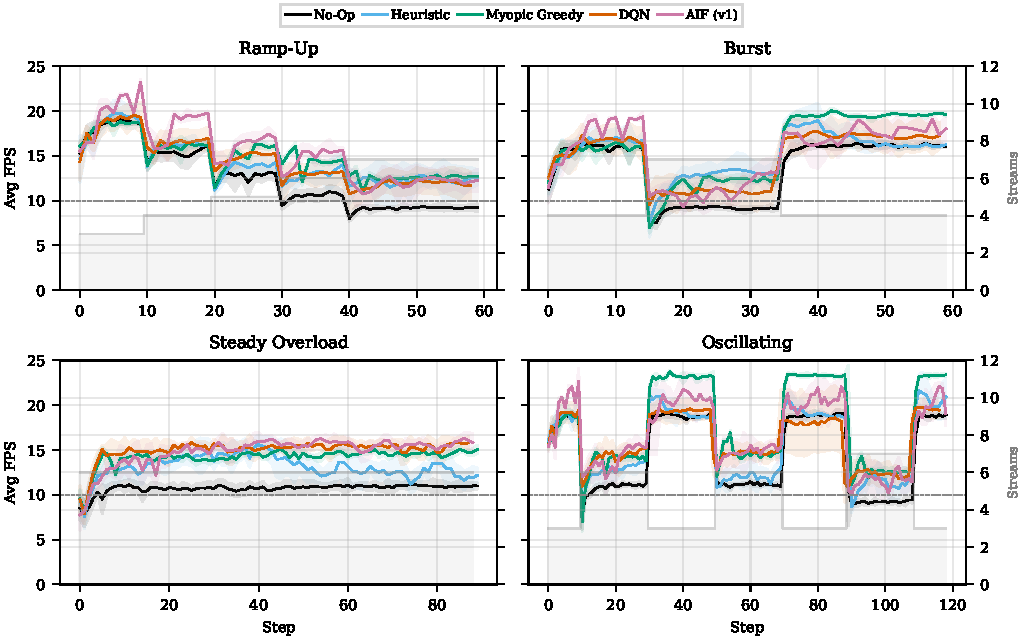
\includegraphics[width=0.94\textwidth]{figures/fig_four_scenario_fps.pdf}
\end{center}
\vspace{-0.35cm}
\begin{columns}[c]
  \begin{column}{0.23\textwidth}\centering\small
    \textbf{Ramp-up}\\3\,$\to$\,7 streams, 60\,s
  \end{column}
  \begin{column}{0.23\textwidth}\centering\small
    \textbf{Burst}\\spike at $t$\,=\,15\,s,\\drop at $t$\,=\,35\,s
  \end{column}
  \begin{column}{0.23\textwidth}\centering\small
    \textbf{Steady Overload}\\6 streams fixed, 90\,s
  \end{column}
  \begin{column}{0.23\textwidth}\centering\small
    \textbf{Oscillating}\\three successive\\add/remove waves
  \end{column}
\end{columns}
\end{frame}

% ---- 8. Main results ----------------------------------------------------
\begin{frame}{Main Results}
\begin{columns}[T]
  \begin{column}{0.57\textwidth}
    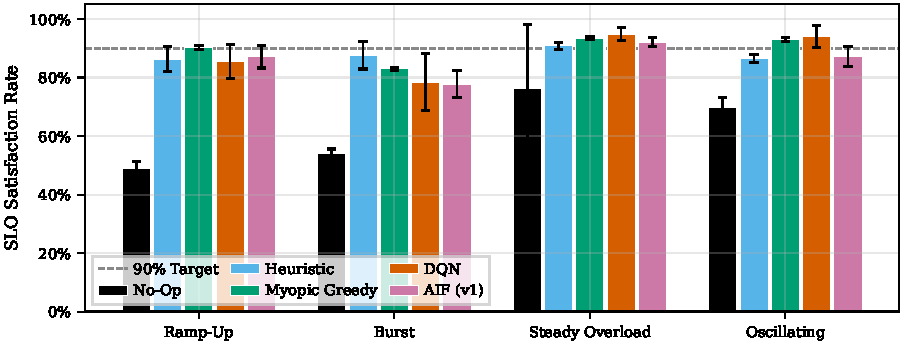
\includegraphics[width=\textwidth]{figures/fig_slo_bar.pdf}
  \end{column}
  \begin{column}{0.40\textwidth}
    \vspace{0.15cm}
    \small
    \begin{tabular}{@{}lc@{}}
      \toprule
      Controller & Avg SLO \\
      \midrule
      No-Op     & 62.2\% \\
      Heuristic & 87.8\% \\
      Myopic Greedy & 89.9\% \\
      DQN       & 88.2\% \\
      \textbf{AIF (v1)} & \textbf{86.0\%} \\
      \bottomrule
    \end{tabular}
    \vspace{0.7em}

    AIF without training data is \textbf{competitive with DQN and Heuristic}.\\[0.5em]

    \textbf{Strongest in steady overload:}\\
    AIF 92.1\% $>$ Heuristic 90.9\%\\
    — structured OFFLOAD usage at 22.8\%.\\[0.5em]

    \textbf{Weakest in burst:}\\
    AIF 77.7\% ($-$9.9\,pp vs.\ Heuristic)\\
    — 3-step cooldown delays reaction.\\[0.5em]

    \textbf{AIF std: 1.4–4.5\%} across all scenarios.
  \end{column}
\end{columns}
\end{frame}

% ---- 9. DQN instability -------------------------------------------------
\begin{frame}{DQN Is Structurally Unpredictable}
\begin{columns}[T]
  \begin{column}{0.58\textwidth}
    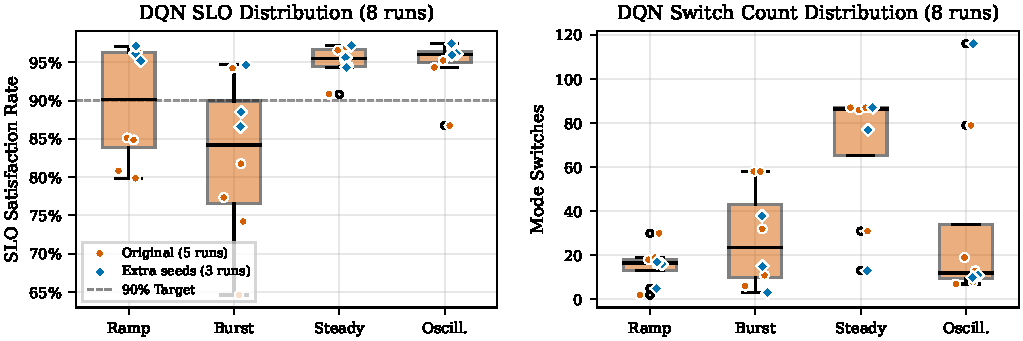
\includegraphics[width=\textwidth]{figures/fig_dqn_variance.pdf}
  \end{column}
  \begin{column}{0.39\textwidth}
    \vspace{0.3cm}
    \small
    8 independent DQN runs\\
    (5-episode training each, retrained from scratch)\\[0.8em]

    \textbf{Burst scenario:}\\[0.3em]
    SLO range:\hspace{0.5em}\textcolor{mywarn}{\textbf{64.6\,\%\,–\,94.3\,\%}}\\[0.2em]
    Switch counts:\hspace{0.2em}\textcolor{mywarn}{\textbf{2\,–\,87}}\\[0.8em]

    This is not measurement noise.\\
    It's structural instability from under-training.\\[0.8em]

    5 episodes isn't enough to produce\\
    a reliable policy in a dynamic environment.\\[0.8em]

    \textbf{AIF std $\leq$ 4.5\%}\\
    Same hardware. No training.
  \end{column}
\end{columns}
\end{frame}

% ---- 10. Key finding — ablation -----------------------------------------
\begin{frame}{The Key Finding — Model Spec Dominates Tuning}
\begin{columns}[T]
  \begin{column}{0.52\textwidth}
    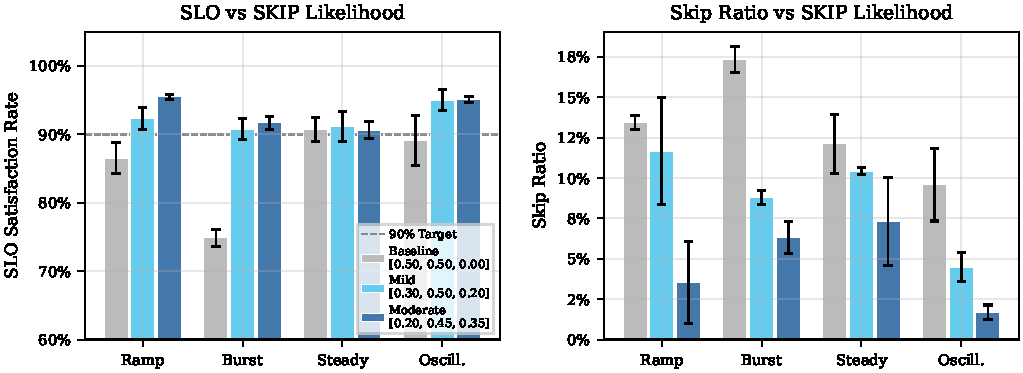
\includegraphics[width=\textwidth]{figures/fig_skip_likelihood.pdf}
  \end{column}
  \begin{column}{0.45\textwidth}
    \vspace{0.2cm}
    \small
    \textbf{Isolated effect of each likelihood correction:}\\[0.4em]
    \begin{tabular}{@{}lcccc@{}}
      \toprule
      Correction & Base & After & $\Delta$ \\
      \midrule
      OFFLOAD v0\,$\to$\,v1   & 78.8\% & 86.7\% & \textbf{+7.9} \\
      SKIP neutral\,$\to$\,mod.& 85.3\% & 93.2\% & \textbf{+7.9} \\
      \midrule
      Both corrections         & 78.8\% & \textbf{93.2\%} & \textbf{+14.4} \\
      \bottomrule
    \end{tabular}
    \vspace{0.7em}

    vs.\ all secondary hyperparameters combined:\\[0.2em]
    \hspace{1em}$\beta$ (precision) + $w_e$ + cooldown
                                    $<$ \textbf{8\,pp}\\[0.8em]

    \textcolor{mygreen}{\textbf{Likelihood corrections: $\sim$2$\times$ the tuning contribution.}}\\[0.5em]

    \textit{Model construction, not algorithmic tuning,\\
    is the dominant challenge for AIF deployment.}
  \end{column}
\end{columns}
\end{frame}

% ---- 11. AIF belief dynamics --------------------------------------------
\begin{frame}{AIF Decides Proactively — Belief Dynamics}
\begin{columns}[T]
  \begin{column}{0.58\textwidth}
    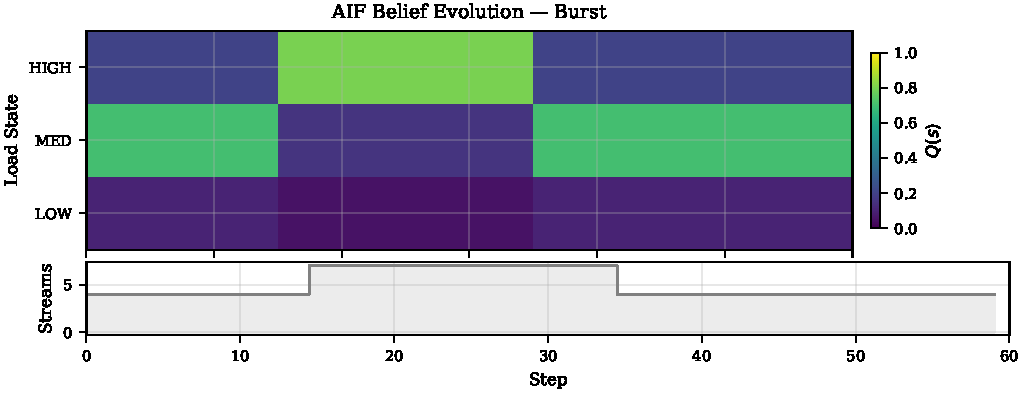
\includegraphics[width=\textwidth]{figures/fig_belief_scenario_burst.pdf}
  \end{column}
  \begin{column}{0.39\textwidth}
    \vspace{0.3cm}
    \small
    \textit{Burst: 4 streams stable, 3 added at step\,15, removed at step\,30}\\[0.8em]

    The belief $Q(s)$ tracks the true load state\\
    \textbf{without observing it directly.}\\[0.5em]

    Step 15 (streams spike):\\
    $p_\textsc{High}$ rises rapidly — controller\\
    switches to OFFLOAD \emph{before}\\
    visible SLO violations accumulate.\\[0.5em]

    Step 30 (streams drop):\\
    Belief shifts back to MED/LOW.\\
    Controller relaxes.\\[0.8em]

    This is the transparency property\\
    DQN doesn't have:\\[0.3em]
    \textbf{inspect $Q(s)$ and EFE at each step\\
    to understand why an action was chosen.}
  \end{column}
\end{columns}
\end{frame}

% ---- 12. AIF mode allocation --------------------------------------------
\begin{frame}{What AIF Actually Decides — Mode Allocation}
\begin{columns}[T]
  \begin{column}{0.63\textwidth}
    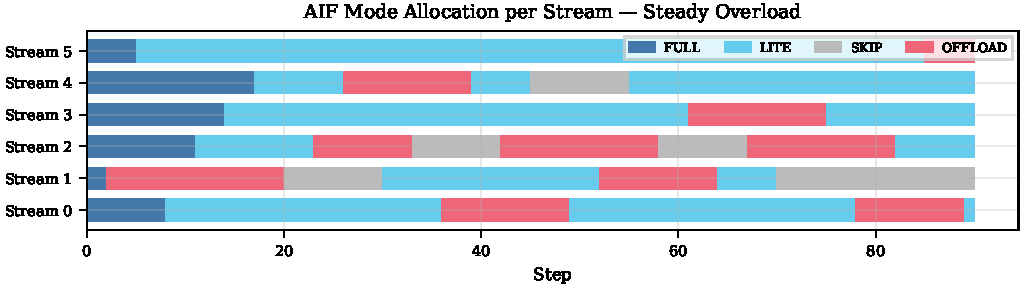
\includegraphics[width=\textwidth]{figures/fig_gantt_scenario_steady_overload.pdf}
  \end{column}
  \begin{column}{0.34\textwidth}
    \vspace{0.3cm}
    \small
    \textit{Steady overload: 6 streams throughout 90\,s}\\[0.8em]

    FULL (dark blue): brief initial period\\
    LITE (cyan): dominant mode\\
    OFFLOAD (red): rotated across streams\\
    SKIP (gray): used sparingly\\[0.8em]

    AIF dynamically balances load\\
    across all 6 streams without\\
    a single stream being\\
    permanently SKIPped.\\[0.8em]

    Offload ratio: \textbf{22.8\%}\\
    This is \textbf{cluster-level} thinking\\
    — not per-stream reaction.
  \end{column}
\end{columns}
\end{frame}

% ---- 13. Takeaways ------------------------------------------------------
\begin{frame}{Takeaways}
\begin{columns}[T]
  \begin{column}{0.47\textwidth}
    \vspace{0.1cm}
    \begin{block}{Key 1 — It's a POMDP}
      \small
      FPS and latency are noisy proxies.\\
      GPU contention, thermal throttling, queue depth\\
      are hidden.\\[0.3em]
      Threshold rules can't reason under this uncertainty.\\
      Belief-based control can.
    \end{block}
    \vspace{0.35em}
    \begin{block}{Key 2 — Model Semantics Are the Method}
      \small
      OFFLOAD and SKIP likelihood corrections\\
      (+7.9\,pp each) outweigh all hyperparameter\\
      effects combined ($<$8\,pp).\\[0.3em]
      \emph{How you encode actions matters more\\
      than which algorithm you use.}
    \end{block}
    \vspace{0.35em}
    \begin{block}{Key 3 — Predictability Over Peak Performance}
      \small
      AIF: no training, std\,$\leq$\,4.5\%.\\
      DQN burst: 64\%–94\% across seeds.\\[0.3em]
      For deployments where \emph{reliability matters}.
    \end{block}
  \end{column}

  \begin{column}{0.50\textwidth}
    \vspace{0.1cm}
    \begin{alertblock}{Open Question — Can the Agent Learn Its Own Semantics?}
      \small
      \vspace{0.2em}
      Right now, OFFLOAD and SKIP likelihoods\\
      come from static hardware profiling.\\[0.5em]
      What if we treat the likelihood matrices as\\
      \textbf{latent variables} subject to Bayesian inference?\\[0.5em]
      Parameter learning in the full AIF framework\\
      would let the scheduler \emph{discover} the\\
      system-level effects of each action\\
      through experience — no profiling needed.\\[0.5em]
      \textbf{This is the primary direction for\\
      follow-on work.}
      \vspace{0.2em}
    \end{alertblock}
    \vspace{0.5em}
    \small
    \textcolor{mygray}{
      EDCCS 2026 @ ICDCS, Seoul, June 2026\\[0.2em]
      Contact: \texttt{[email]}
    }
  \end{column}
\end{columns}
\end{frame}

\end{document}
